\def\pgfsysdriver{pgfsys-dvisvgm.def}
% flashcards-title: Iterative map of scientific inquiry
% flashcards-desc: Boxes for observations, questions, hypotheses, predictions, comparisons, and revision are connected by forward and return arrows.
\documentclass[tikz,border=6pt]{standalone}
\usetikzlibrary{arrows.meta,calc,fit,positioning,shapes.geometric}

\definecolor{fcink}{HTML}{17212B}
\definecolor{fcblue}{HTML}{1D5D8C}
\definecolor{fcgreen}{HTML}{2D6A4F}
\definecolor{fcorange}{HTML}{A44A1F}
\definecolor{fcpale}{HTML}{F4F7F9}
\definecolor{fcsoil}{HTML}{8B5E3C}

\tikzset{
  fc text/.style={font=\sffamily, text=fcink},
  fc panel/.style={draw=fcink, line width=0.9pt, rounded corners=5pt, fill=fcpale},
  fc node/.style={draw=fcink, line width=0.9pt, rounded corners=4pt, fill=white,
    minimum width=24mm, minimum height=10mm, align=center, font=\sffamily},
  fc arrow/.style={-{Stealth[length=3.2mm,width=2.4mm]}, line width=1.2pt,
    draw=fcblue, line cap=butt},
  fc boundary/.style={draw=fcorange, line width=1.4pt, dash pattern=on 5pt off 3pt,
    rounded corners=7pt},
  fc label/.style={font=\sffamily\bfseries, text=fcink},
  fc note/.style={font=\sffamily\small, text=fcink, align=center}
}

\begin{document}
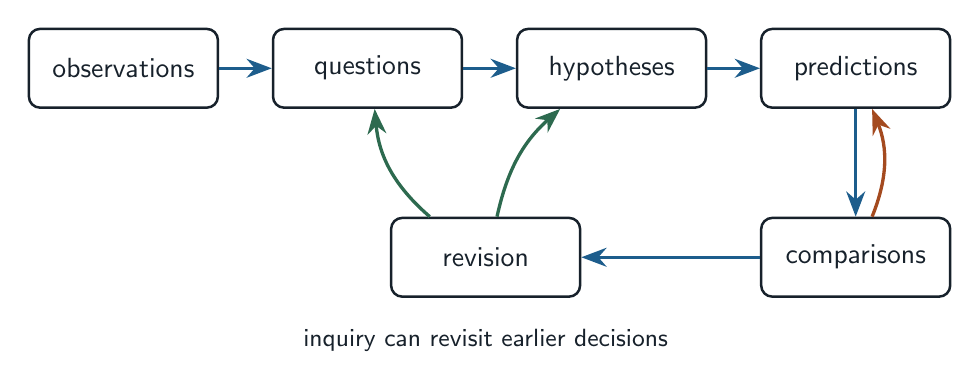
\begin{tikzpicture}[fc text, x=1cm, y=1cm]
  \node[fc node] (o) at (1.6,3.7) {observations};
  \node[fc node] (q) at (4.7,3.7) {questions};
  \node[fc node] (h) at (7.8,3.7) {hypotheses};
  \node[fc node] (p) at (10.9,3.7) {predictions};
  \node[fc node] (c) at (10.9,1.3) {comparisons};
  \node[fc node] (r) at (6.2,1.3) {revision};
  \draw[fc arrow] (o)--(q);
  \draw[fc arrow] (q)--(h);
  \draw[fc arrow] (h)--(p);
  \draw[fc arrow] (p)--(c);
  \draw[fc arrow] (c)--(r);
  \draw[fc arrow, draw=fcgreen, bend left=18] (r) to (h);
  \draw[fc arrow, draw=fcgreen, bend left=22] (r) to (q);
  \draw[fc arrow, draw=fcorange, bend right=22] (c) to (p);
  \node[fc note] at (6.2,0.25) {inquiry can revisit earlier decisions};
\end{tikzpicture}
\end{document}
